\chapter{Implementation \& System Architecture}
\label{chap:implementation}

This chapter details the design and implementation of the prototype system, a practical realization of the conceptual framework for \gls{genai}-driven security automation introduced in Chapter~\ref{chap:conceptual_framework}. The work is implemented through two distinct but interconnected codebases: a cloud-native infrastructure for the \gls{genai} backend, and a Python-based application that orchestrates the analysis and \gls{pg} workflow.

The primary goal of this implementation is to empirically validate the central hypothesis of the theoretical framework: that a hybrid approach, combining traditional static analysis with advanced \gls{llm} capabilities, can significantly enhance the automation of security \gls{pg} for \gls{iac}. This chapter will demonstrate how the system architecture directly maps to the four-layered conceptual model Data Ingestion, Data Processing, Code Generation, and Validation. It will further illustrate how this architecture realizes the core principles of leveraging \gls{rag} for contextual accuracy and integrating a \gls{hitl} for safety and oversight.

We will first present the high-level architecture and the technology stack chosen to satisfy the functional requirements of a robust, scalable, and reproducible security pipeline. Subsequently, the chapter will provide a detailed examination of both the cloud infrastructure, deployed via \gls{terraform}, and the Python prototype, focusing on the specific modules that implement the core logic of the system. The chapter will conclude by illustrating the end-to-end workflow, from the initial analysis of a \gls{terraform} file to the generation and validation of a corresponding Rego security policy, thereby providing a comprehensive account of the system's practical application.

\section{Design Objectives \& Functional Requirements}

% Refined Research Questions:

%    * RQ1 (Effectiveness and Automation): How can Generative AI technologies be effectively leveraged to automate security policy generation and management across
%      hyperscale cloud platforms?
%    * RQ2 (Architecture and Orchestration): What specific architectural patterns and validation mechanisms are required to ensure trust, accuracy, and effective
%      multi-cloud orchestration in GenAI-driven security automation?
%    * RQ3 (Measurement and Validation): How can the effectiveness of GenAI-driven security automation be quantitatively measured and validated, particularly in terms
%      of accuracy, reliability, and efficiency gains?
%    * RQ4 (Human-in-the-Loop): What is the optimal balance between automation and human oversight (Human-in-the-Loop) to maximize security outcomes and mitigate the
%      risks of GenAI-driven policy generation?

%   These questions are more closely aligned with the language and focus of your exposé.

The practical implementation of the prototype is guided by a set of specific design objectives and functional requirements. These objectives are derived directly from the core research questions and serve to translate the high-level scientific inquiry into concrete, measurable goals for the system. The following objectives define the core functionality of the prototype:

\begin{itemize}
\item \textbf{Automated, High-Fidelity Policy Generation:} The system's primary function is to automatically generate syntactically correct and logically sound security policies in the Rego language from vulnerabilities found in \gls{terraform} files. This objective directly addresses the central research question on the effectiveness of \gls{genai} for security automation \textbf{(RQ1)}. A key requirement is to achieve high fidelity, with a target of $\geq$ 95\% of generated policies being effective in mitigating the identified vulnerability, providing a core metric for validation \textbf{(RQ3)}.
text
\item \textbf{Hybrid and Reproducible Analysis Architecture:} The system is built on a hybrid analysis model that is both reproducible and architecturally sound. Reproducibility is achieved by defining the entire \gls{cloud-native} backend as code using \gls{terraform}. The analysis engine is hybrid, combining traditional \gls{sast} for baseline coverage with \gls{genai}-driven contextual analysis for deeper insights. These architectural choices are fundamental to investigating how to build a trustworthy and effective \gls{genai}-driven system \textbf{(RQ2)}.

\item \textbf{Automated Validation:} To ensure the reliability of the AI-generated artifacts, the system implements a multi-stage, automated validation pipeline. This process checks generated policies for syntactic correctness and performs a security self-scan to ensure they do not introduce new vulnerabilities. This automated validation is a critical mechanism for measuring and ensuring the trustworthiness of the output \textbf{(RQ3)}.

\item \textbf{\gls{hitl} and \gls{cicd} Integration:} The prototype is designed for seamless integration into a standard \gls{cicd} pipeline, where it can act as an automated quality gate. This integration must also support a \gls{hitl} workflow, enabling human review and approval of generated policies. This dual requirement is designed to explore the optimal balance between full automation and necessary human oversight in a practical \gls{devsecops} environment \textbf{(RQ4, RQ1)}.
\end{itemize}

This structured set of objectives ensures that the implementation of the prototype directly and comprehensively contributes to answering the core research questions of this thesis.

\section{Technology \& Tooling Stack}

The selection of the technology and tooling stack for this project was a deliberate process, guided by the design objectives of creating a reproducible, scalable, and industry-relevant prototype. The choices reflect a modern, \gls{cloud-native} approach, emphasizing managed services and open standards to validate the conceptual framework effectively. This section briefly justifies the key technologies that constitute the system's foundation. The chosen stack is summarized in Table~\ref{tab:tech_stack}.

\begin{center}
\begin{tabular}{|l|l|p{7cm}|}
\hline
\textbf{Component} & \textbf{Technology} & \textbf{Justification} \\
\hline
Cloud Platform & \gls{aws} & As the leading hyperscale cloud provider, \gls{aws} offers a mature and extensive ecosystem of services, robust \gls{api}s, and comprehensive documentation. Its managed AI service, AWS Bedrock, is central to the project's architecture. \\
\hline
\gls{genai} Service & \gls{aws} Bedrock \cite{noauthor_claude_nodate} & Provides \gls{api} access to a variety of high-performance foundation models without the operational overhead of self-hosting. This aligns with the objective of a fully-managed \gls{genai} pipeline and allows the research to focus on application logic rather than \gls{mlops}. The Anthropic Claude model was selected for its advanced reasoning capabilities and large context window. \\
\hline
\gls{iac} & HashiCorp \gls{terraform} \cite{noauthor_terraform_nodate} & As the de-facto industry standard for \gls{iac}, \gls{terraform}'s declarative syntax and cloud-agnostic nature ensure the approach is both reproducible and broadly applicable. It is the input format for the security analysis pipeline. \\
\hline
\gls{pac} & \gls{opa} (Rego) \cite{noauthor_introduction_nodate} & The \gls{opa} is a CNCF-graduated project and a general-purpose policy engine. Its declarative language, \gls{rego}, is purpose-built for expressing policies over complex \gls{json}/\gls{yaml} data, making it an ideal target for generating preventative controls for \gls{iac}. \\
\hline
\gls{orchestration} & Python 3.12 \cite{noauthor_whats_nodate} & Python's extensive ecosystem, including the Boto3 library for \gls{aws}, and its strength in scripting and automation makes it the ideal choice for orchestrating the multi-stage workflow, which involves invoking external scanners, calling cloud \gls{api}s, and managing file I/O. \\
\hline
\gls{cicd} & \gls{github} \cite{noauthor_github_2025} & Provides a tightly integrated platform for version control and workflow automation. It enables the seamless implementation of a \gls{cicd} pipeline to trigger scans, orchestrate the policy generation and validation, and manage the \gls{hitl} approval process. \\
\hline
\end{tabular}
\captionof{table}{Technology and Tooling Stack}
\label{tab:tech_stack}
\end{center}

\section{High-Level Architecture}

This section presents the high-level architecture of the \gls{genai}-driven security automation framework. The design translates the conceptual model from Chapter~\ref{chap:conceptual_framework} into a concrete system that orchestrates static analysis tools, \gls{genai}, and validation workflows. The architecture, previously illustrated in the component diagram (Figure~\ref{fig:prototype-architecture}), is realized as a sequential data pipeline that operationalizes the four-layered conceptual model.

The system's responsibilities are segregated into four logical tiers, directly corresponding to the layers of the conceptual framework. The process begins at the Data Ingestion Layer, which serves as the entry point, receiving \gls{terraform} configurations from a \gls{cicd} trigger, parsing the \gls{iac} files, and preparing them for analysis. From there, the artifacts are passed to the Data Processing Layer, the core analysis engine. This layer first subjects the \gls{iac} to a baseline scan using a traditional \gls{sast} tool (Checkov) to identify known vulnerability patterns. The resulting report, along with the original \gls{iac}, is then fed into the \gls{genai} Analysis Engine (\gls{aws} Bedrock) for a deep, contextual analysis to identify complex misconfigurations and reduce \glspl{false-positive}. Subsequently, the Code Generation Layer takes the enriched vulnerability report as input, queries the \gls{rag}-enabled knowledge base for relevant security best practices, and prompts the \gls{llm} via the \gls{aws} Bedrock \gls{api} to generate a corresponding \gls{rego} policy. Finally, the Validation Layer acts as a quality gate. Here, the newly generated \gls{rego} policy is subjected to automated checks, including syntax validation with the \gls{opa} parser and a security self-scan, before being presented to the \gls{hitl} for final approval.

This layered architecture ensures a clear separation of concerns and provides a robust, end-to-end workflow for translating identified risks in \gls{iac} into validated, enforceable security policies.

\section{Cloud-Infrastructure Codebase (IaC)}

The cloud infrastructure that underpins the \gls{genai} backend is defined entirely as code, following modern \gls{iac} principles to ensure reproducibility, security, and maintainability \cite{dasari_infrastructure_2025}. The design is centered on a modular architecture, automated lifecycle management, and robust security controls.

The codebase is structured using a modular \gls{terraform} approach, where the system is decomposed into discrete, reusable modules. Each module encapsulates a core architectural component: a dedicated module for the vector database, another for the \gls{s3} bucket that forms the \gls{rag} knowledge base, and a third for the \gls{aws} Bedrock service itself. This modularity, a cornerstone of scalable \gls{iac}, simplifies management and allows for independent testing and versioning of each component \cite{howard_terraform_2022}.

A key aspect of the architecture is the management of the \gls{genai}'s knowledge and instructions. The \gls{sp}, which provides the \gls{llm} with its core instructions and persona, is externalized into a dedicated system\_prompt.txt file. This separation of concerns is critical, as it allows for the prompt to be version-controlled and iterated upon independently from the infrastructure code. This practice of "prompt engineering" is central to refining the \gls{ai}'s output without altering the system's architecture. The \gls{rag} \gls{kb} itself is implemented using an \gls{s3} bucket, which stores a curated collection of documents. This includes security best practice guides, vulnerability documentation, and technical manuals for the target technologies (e.g., \gls{terraform} and \gls{rego}). This design choice is strategic: it allows the \gls{kb} to be easily updated with new threat intelligence or standards, thereby keeping the \gls{ai}'s responses grounded in current, factual information without the need for costly model fine-tuning \cite{lewis_retrieval-augmented_2021}.

Security is integrated throughout the \gls{iac} design, following the principle of least privilege. \gls{iam} roles and policies are narrowly scoped to grant each component only the permissions necessary for its function. All data, both at rest in the \gls{s3} bucket and in transit, is encrypted using \gls{kms}, and logging is enabled across all services to provide a comprehensive audit trail, adhering to the \gls{srm} \cite{noauthor_aws_nodate}.

The entire lifecycle of this infrastructure is automated via \gls{github} Actions, implementing a GitOps workflow. The \gls{cicd} pipeline handles the provisioning and updating of the environment, ensuring that the deployed infrastructure always reflects the state defined in the main branch of the repository. This automated deployment workflow guarantees consistency and environment parity, forming a reliable foundation for the prototype's operation \cite{noauthor_gitops_nodate}.

\section{Prototype Application Codebase (Python)}

The Python application serves as the \gls{orchestration} engine for the entire \gls{security-automation} framework. It is designed as a command-line tool that implements the logic of the multi-layered conceptual model, connecting the static analysis, \gls{genai}, and validation stages into a cohesive workflow. The codebase adheres to modern software engineering best practices, emphasizing modularity, clear separation of concerns, and robust quality assurance.

The application's architecture is inherently modular, with functionality partitioned into distinct, single-responsibility components. This design enhances maintainability and testability \cite{martin_clean_2009}. The core modules include:

\begin{itemize}
    \item An \textbf{Analyzer} module, which acts as an adapter for the underlying \gls{sast} tool (Checkov). It is responsible for invoking the scanner on a given \gls{terraform} file and normalizing the output into a standardized data structure for consumption by the rest of the application.
    \item A \textbf{Policy Generation} module, which represents the core intelligence of the system. This component orchestrates the interaction with the \gls{genai}. It constructs a detailed, context-rich prompt by combining the findings from the analyzer with relevant information retrieved from the \gls{rag} \gls{kb}. It then communicates with the \gls{aws} Bedrock \gls{api} to obtain the generated \gls{rego} policy.
    \item A \textbf{Validator} module, which functions as an automated quality gate for the \gls{ai}-generated artifact. It performs crucial checks to ensure the reliability of the output, primarily by using the \gls{opa} toolchain to validate the syntactic correctness of the generated \gls{rego} code.
\end{itemize}

A main control loop in the application's entry point script (`main.py`) orchestrates these modules in sequence, executing the end-to-end process from analysis to generation and validation.

To ensure code quality and the reliability of the prototype, a comprehensive testing strategy is employed. The project utilizes the pytest framework to implement a suite of unit tests that verify the functionality of each module in isolation \cite{noauthor_pytest_nodate}. Fixtures are used to create consistent and reusable test setups, and test coverage is monitored as a quality gate within the \gls{cicd} pipeline. Furthermore, dependency management is handled through a ''requirements.txt'' file, which pins the specific versions of all external libraries. This practice guarantees a reproducible and stable runtime environment, which is critical for consistent behavior and scientific validation.

\section{End-to-End Workflow}

The practical application of the framework is best understood by examining the end-to-end workflow of the command-line tool. This process describes the sequence of operations from the moment a user invokes the application to the final output of a validated security policy. The entire sequence is designed to be a self-contained, automated process, as illustrated in the sequence diagram \ref{fig:e2e_workflow}.

The sequence diagram depicts the temporal flow of interactions between the key actors in the system: the User, the Python Command-Line Application, and the external services (Checkov, \gls{aws} Bedrock, and \gls{opa}). The diagram illustrates how control and data flow through the system in a step-by-step manner, beginning with the user's command-line invocation and proceeding through each processing stage. The vertical lifelines represent the different system components, while the horizontal arrows show the sequence of method calls, \gls{api} requests, and data exchanges. This visualization clearly demonstrates the \gls{orchestration} role of the Python application as it coordinates between traditional security tools, cloud-based \gls{ai} services, and validation frameworks to deliver a comprehensive security policy generation workflow.

\begin{landscape}
\thispagestyle{empty}
\begin{figure}[p]
\centering
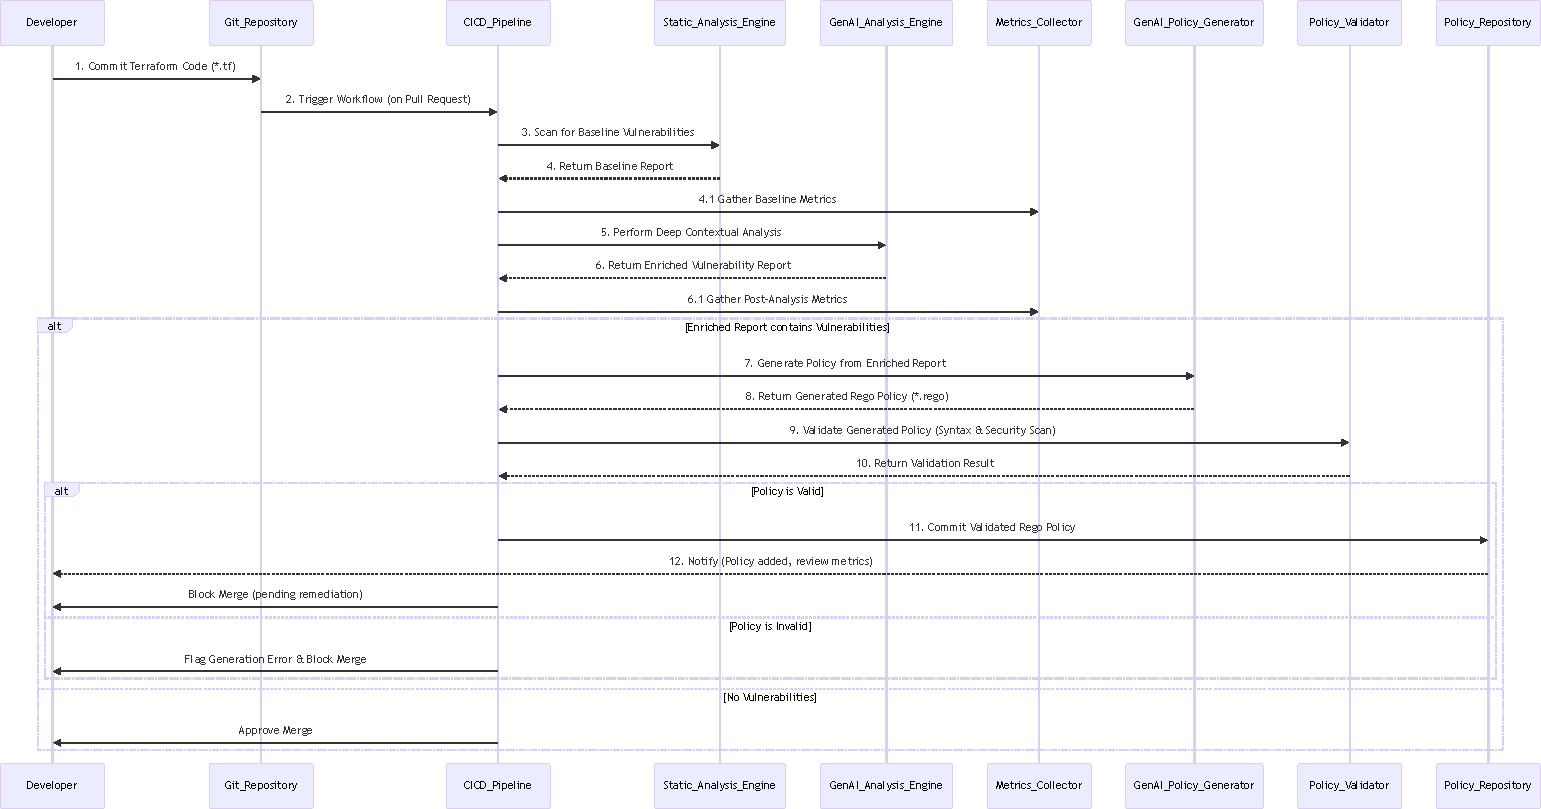
\includegraphics[width=0.9\linewidth,height=0.7\textheight,keepaspectratio]{Figures/image.pdf}
\caption{End-to-End Workflow Sequence Diagram}
\label{fig:e2e_workflow}
\end{figure}
\end{landscape}

The workflow is initiated when a user executes the main Python script from the command line, providing the path to a target Terraform (`.tf`) file as an argument. The application then proceeds through the following automated steps:

\begin{enumerate}
    \item \textbf{Static Scan:} The \textbf{Analyzer} module is invoked. It runs the Checkov \gls{sast} tool on the specified \gls{terraform} file to identify any known misconfigurations or vulnerabilities.
    \item \textbf{GenAI Contextual Analysis:} The structured findings from the static scan are fed into the \gls{genai} Analysis Engine (\gls{aws} Bedrock) for deep, contextual analysis to reduce \glspl{false-positive} and identify complex misconfigurations that traditional tools might miss.
    \item \textbf{Policy Generation:} The enriched vulnerability report from the \gls{genai} analysis is passed to the \gls{pg} module. This component constructs a detailed, context-rich prompt by combining the analysis findings with relevant information retrieved from the \gls{rag} \gls{kb}, then communicates with the \gls{aws} Bedrock \gls{api} to generate a targeted \gls{rego} policy specifically designed to mitigate the identified risks.
    \item \textbf{Validation:} The raw, generated \gls{rego} policy is immediately passed to the \textbf{Validator} module. This component uses the \gls{opa} toolchain to verify that the policy is syntactically correct and well-formed.
    \item \textbf{Output:} If the policy successfully passes validation, the application saves the new Rego policy as a `.rego` file to a designated output directory. The application's execution concludes by printing the path to the generated file to the console.
\end{enumerate}

This self-contained workflow from file input to policy output is designed for both interactive use by a security analyst and for integration into larger automated systems. For example, it can be executed as a script within a \gls{cicd} pipeline, where the resulting policy artifact can then be automatically committed to a repository and used as a quality gate.

\section{CI/CD \& DevSecOps Integration}

While the prototype is a self-contained command-line tool, its primary intended application is within a \gls{cicd} pipeline to enable a proactive \gls{devsecops} workflow. This integration automates the process of security analysis and policy enforcement, "shifting left" to catch and remediate vulnerabilities before they reach production \cite{delicheh_mitigating_2024}. The implementation uses \gls{github} Actions as the \gls{cicd} platform.

The integration is achieved through a \gls{github} Actions workflow that is triggered whenever a developer opens a pull request containing changes to \gls{terraform} files. This workflow acts as an automated quality gate and performs the following steps:

\begin{enumerate}
    \item \textbf{Code Checkout \& Setup:} The pipeline begins by checking out the source code and setting up the Python environment, including installing the dependencies from ''requirements.txt''.
    \item \textbf{Execute Security Scan:} The core command-line application is executed. It is pointed at the modified Terraform files within the pull request, running the end-to-end workflow of scanning, generation, and validation.
    \item \textbf{Commit New Policy:} If the tool successfully generates a new, validated Rego policy, the workflow commits this new policy file to a dedicated directory within the repository.
    \item \textbf{Enforce Policy as a Quality Gate:} The pipeline then uses the \gls{opa} toolchain to evaluate the proposed \gls{terraform} changes against the entire set of \gls{rego} policies in the repository, including the one that was just generated. If the proposed changes violate any policy, the \gls{opa} evaluation fails.
    \item \textbf{Block or Approve:} A failure in the \gls{opa} evaluation causes the entire \gls{cicd} pipeline to fail. This automatically blocks the pull request from being merged and provides immediate feedback to the developer that their changes are not compliant with security standards. This gating mechanism ensures that only secure and compliant \gls{iac} can be merged into the main branch.
\end{enumerate}

By integrating the command-line tool in this manner, the framework moves from being a simple analysis utility to a powerful, automated control that is seamlessly embedded in the software development lifecycle.

\section{Observability \& Runtime Telemetry}
% Metrics (MTTD, policy-generation latency), structured logging (JSON Logs + AWS CloudWatch), dashboards.

\section{Limitations \& Trade-offs}
% Model latency vs. cost, Terraform state confidentiality, policy false-negatives, Bedrock service quotas.

\section{Summary}
% Recap key design choices and link forward to the Results chapter.